\documentclass[conference]{IEEEtran}
\IEEEoverridecommandlockouts
% The preceding line is only needed to identify funding in the first footnote. If that is unneeded, please comment it out.
\usepackage{cite}
\usepackage{amsmath,amssymb,amsfonts}
\usepackage{algorithmic}
\usepackage{graphicx}
\usepackage{textcomp}
\usepackage{xcolor}
\def\BibTeX{{\rm B\kern-.05em{\sc i\kern-.025em b}\kern-.08em
    T\kern-.1667em\lower.7ex\hbox{E}\kern-.125emX}}
\begin{document}

\title{Real-time Domain Adaptation in Semantic Segmentation*\\
{\footnotesize \textsuperscript{*}Note: Sub-titles are not captured in Xplore and
should not be used}
}

\author{\IEEEauthorblockN{1\textsuperscript{st} Berardo Nicholas}
\IEEEauthorblockA{\textit{dept. Computer Engineering} \\
\textit{Politecnico di Torino}\\
Turin, Italy \\
s319349@studenti.polito.it}
\and
\IEEEauthorblockN{2\textsuperscript{nd} Cardona Riccardo}
\IEEEauthorblockA{\textit{dept. Computer Engineering} \\
\textit{Politecnico di Torino}\\
Turin, Italy \\
s319441@studenti.polito.it}
\and
\IEEEauthorblockN{3\textsuperscript{rd} De Marco Alessando}
\IEEEauthorblockA{\textit{dept. Computer Engineering} \\
\textit{Politecnico di Torino}\\
Turin, Italy \\
sXXXXXX@studenti.polito.it}
}

\maketitle

\begin{abstract}
We use an efficient structure named Short-Term Dense Concatenate network (STDC network) for the semantic segmentation task. This
structre reduce the dimension of feature maps and use the aggregation of them for image representation, then use a Detail aggregation
module for producing the low-level features. Finally these two are merged to produce the segmentation result. We test this model on 
Cityscapes and GTA V, following the evaluation of the domain shift between GTA V and Cityscapes and finally we implement and 
unsupervised adversarial domain adaptation method used for reducing the domain shift. We also show the result for the STDC network in
term of mIoU and the result for the domain adaptation. 
\end{abstract}


\section{Introduction}
Semantic Segmentation is a topic in computer vision that aims at assigning a label to each pixel of the image. This is used in many fields
such as autonomous veichle, video surveillance and robot sensing. There are a lot of models that can achive good accuracy. For real-time
semantic segmentation some models choose lightweight backbones for having an increase of performance but a drastic drop of accuracy. For
this reason some new methods were investigated, like feature fusion or aggregation modules. Other models reduce the input image size 
but this can result in a bad accuracy around boundaries and small object. 

STDC net \cite{b1} uses the first approach. Fig.~\ref{stdc_net} shows how the image is encoded in different scales. The kernel size is also reduced
to speed-up the performance but with an acceptable loss in accuracy. Then a Detail Guidance is used to learn the space details insted of 
using a Spacial Path as in BiSeNet \cite{b2}.

The next step is domain adaptation. A model trained on a certain dataset may not generalize on an unseen dataset ending in poor performance.
This is caused by the domain shift beetween the source (training) and terget (test) dataset, for example different cities, weather and 
lighting conditions. Domain adaptation methods are used to close the gap between source and target domains. In this paper we use an 
adversarial domain adaptation method \cite{b3} that is composed of a segmentation model to predict the output and a discriminator to
predict is the input is from the source or target domain. The goal is to generate a segmentation output from the segmentation part that 
fool the discriminator, meaning that the segmentation output is similar between source and target domains. We show experiments done on 
the adaptation between GTAV and Cityscapes.

Our contributions can be summarized as follows:
First we build the STDC network and train it on Cityscapes and test it again on Cityscapes. Second we reply the same idea over the 
GTAV dataset, so train on GTAV and test on GTAV. Third we compute the domain shift between GTAV (source) and Cityscapes (target) domains
firstly in vanilla, then with some augmentation on GTAV. Fourth we implement the adversarial domain adaptation method and test it 
with GTAV as source domain and Cityscapes as target domain. Lastly we apply some real-time semantic segmentation method to our 
discriminator function in order to make it faster. 


\begin{figure}[tp]
\centerline{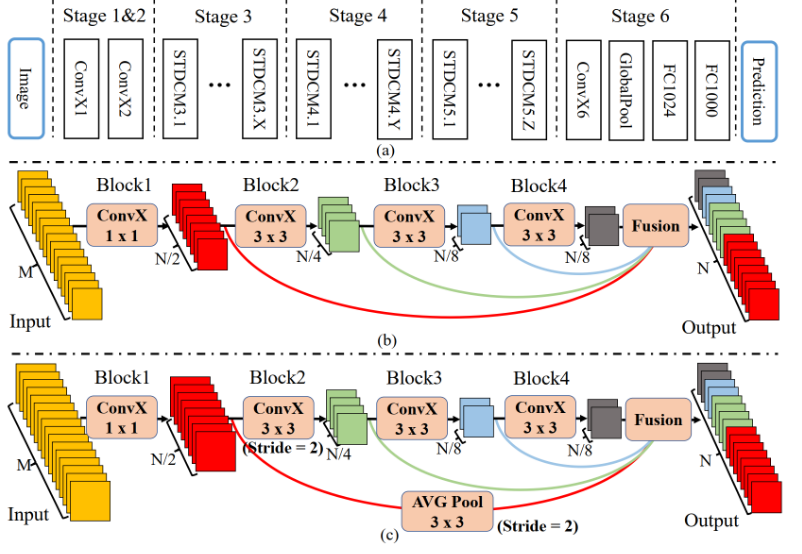
\includegraphics[width=0.4\textwidth]{figures/Figure1-STDCnet.png}}
\caption{STDC network.}
\label{stdc_net}
\end{figure}

\section{Related Word}

Chiedere cosa mettere
\section{Methods}

We first introduce the Short-Term Dense Concatenate network (STDC network) and how we used it with BiSeNet \cite{b2},
then the unsupervised adversarial domain adaptation method.

STDC network \cite{b1} is represented in Fig.~\ref{stdc_net} (a). Stage 3,4 and 5 have a number of Short-Term Dense Concatenate Module (STDCM)
where each module is composed of ConvX blocks Fig.~\ref{stdc_net} (b)(c). Each \(ConvX_i\) is a block composed of one convolutional layer,
one batch normalization layer and one ReLU activation layer. The ConvX layers filter the input into N/2, where N is the channel number
of the STDC module. At the end we concatenate the output of each ConvX block as follow: 
\[x_{output} = F(x_1,x_2,...,x_n)\]
where \(x_{output}\) is the STDC module output, \(F\) is the fusion operation, that in our case is the concatenation and \(x_1,x_2,
...,x_n\) are the output of each \(ConvX_i\) block.

This STDC network is then used as backbone for the context path of BiSeNet, in particular we use stage 3,4 and 5 to reduce the 
feature map to obtain large receptive field. Then a global avarage pooling in added on the tial of the context path. We also use
Attention Refine Module (ARM) on Stage 4 and 5. Finally a Future Fusion Model (FFM) is used to fuse the 1/8
feature from Stage 3 with this last part.

The main idea of the unsupervised adversarial domain adaptation method \cite{b3} is to create a segmentation network that classify the source
image (that as a label) and the target image (without annotations). Then those two predictions are given to the discriminator that
has to distinguish whether the input is from source or target domain. To do so we need a loss from the discriminator to the 
segmentation network which encourage the segmentation to generate similar preditions. We use as segmentation newtork the BiSeNet 
developed above. The loss is 
\[L(I_s,I_t) = L_{seg}(I_s) + \lambda_{adv}*L_{adv}(I_t)\]
where \(L_{seg}\) is the cross entropy loss for the prediction of the source domain, \(\lambda_{adv}\) is the weight used to 
balance the \(L_{adv}\) that is a BCEWithLogitLoss.
We first forward \(I_s\) to the segmentation newtork to get the predition \(P_s\) and the loss \(L_{seg}\) using the label of \(I_s\).
Then forward \(I_t\) to the segmentation network to get the predition \(P_t\) and feed \(P_s\) to the discriminator and get the 
\(L_{adv}\) and optimize the segmentation network. Now let's optimize the discriminator computing first the loss on the GTA5 image
with label 1 and finally computing the loss on the Cityscape image, with label 0. 

Finally we also tried to apply some real-time semanitc segmentation method to our discriminator to make is lighter and faster.
We build a discriminator using depthwise separable convolutions, following MobileNets \cite{b4}. These are composed of two part: 
depthwise convolutions and pointwise convolutions. Depthwise convolutions are used to filter each input channel, but they can
only filter so we use pointwise convolutions (1 x 1 kernel size) to generate new features. Now our discriminator is based on blocks of
depthwise convolution layer, leaky ReLU, pointwise convolution and again leaky ReLU. 

\section{Experiments}

We have done the following experiments: (1) train on Cityscapes and test on Cityscapes, (2) train on GTA5 and test on GTA5, (3) train on 
GTA5 and test on Cityscapes without domain adaptation, (4) train on GTA5 and test on Cityscapes without domain adaptation with some
augmentation on GTA5, (5) train on GTA5 and test on Cityscapes with domain adaptation and (6) train on GTA5 and test on Cityscapes with
domain adaptation with a lighter discriminator. 
We use as optimizer the SGD (Stocastic Gradient Descent) with momentum set at 0.9 and weight decay at \(5e^{-4}\). We use a batch size of 
2 and poly learning rate where the learning rate is updated as follow \(lr = init\_lr * (1 - \frac{iter}{max\_iter})^{power}\), where
\(init\_lr\) is 0.01, \(iter\) is the actual epoch, \(max\_iter\) is the number of epochs and \(power\) is 0.9. Data augmentation, when
used, contains Color Jitter, Random Horizontal Flip, Random Crop and Normalization. The disciminator for the domain apadtation part
is trained using Adam with a poly learning rate with the same parameter as before. 
We perform our experiments with those versions:\textbf{TODO!!!!!!!!!}

(1) Here we trained our model on Cityscapes train set and test it on Cityscapes validation set. Here there's no domain adaptation, so
we expect to have high results. Table~\ref{CityscapesToCityscapes} shows the results.

(2) We train our model on GTA5 train set and test it on GTA5 validation set. Again we expect high results.  
Table~\ref{GTATOGTA} shows the results.

(3) Here we evaluate the domain shift between GTA5 and Cityscapes. We train on GTA5 train set and test on Cityscapes validation set.
Here we don't have any domain adaptation method, so we expect bad results. Table~\ref{GTATOCITYSCAPESNOADAP} shows the results. We can 
see that the mIoU is low, this because the source domain and target domain are different. 

(4) Again we evaluate the domain shift between GTA5 and Cityscapes, but this time with some augmentation on GTA5. Table~\ref{GTATOCITYSCAPESNOADAPAUG}
shows the results and again the mIoU is low beacause of the domain shift, but higher than step (3). This thanks to the augmentation 
done on GTA5.

(5) Here we have domain adaptation \cite{b3}. So we train on GTA5 and test on Cityscapes, but this time we train also the discriminator
with the segmentation network. Table~\ref{GTATOCITYSCAPESADAP} shows the results. We can see a slight improvement of performance
in the mIoU of 3\% with respect to (4).

(6) Finally we implement depthwise separable convolutions in the discriminator. Again same thing as (5) but with a lighter discriminator. Table
~\ref{GTATOCITYSCAPESADAPLIGHT} shows the results. 



\begin{table}[tb]
\caption{Train on Cityscapes train set and test it Cityscapes val set}
\begin{center}
\begin{tabular}{|c|c|c|}
\hline
\multicolumn{3}{|c|}{\textbf{Cityscapes -$>$ Cityscapes}} \\
\cline{1-3} 
\textbf{\textit{Accuracy (\%)}}& \textbf{\textit{mIoU (\%)}}& \textbf{\textit{Train time (avg per-epoch)}} \\
\hline
81.1& 58.6& 2.5 minutes   \\
\hline
\end{tabular}
\label{CityscapesToCityscapes}
\end{center}
\end{table}

\begin{table}[tb]
\caption{Train on GTA5 train set and test it GTA5 val set}
\begin{center}
\begin{tabular}{|c|c|c|}
\hline
\multicolumn{3}{|c|}{\textbf{GTA5 -$>$ GTA5}} \\
\cline{1-3} 
\textbf{\textit{Accuracy (\%)}}& \textbf{\textit{mIoU (\%)}}& \textbf{\textit{Train time (avg per-epoch)}} \\
\hline
80.82& 62.36& 3,4 minutes   \\
\hline
\end{tabular}
\label{GTATOGTA}
\end{center}
\end{table}

\begin{table}[tb]
\caption{Train on GTA5 train set and test it Cityscapes val set without adaptation}
\begin{center}
\begin{tabular}{|c|c|c|}
\hline
\multicolumn{3}{|c|}{\textbf{GTA5 -$>$ Cityscapes}} \\
\cline{1-3} 
\textbf{\textit{Accuracy (\%)}}& \textbf{\textit{mIoU (\%)}}& \textbf{\textit{Train time (avg per-epoch)}} \\
\hline
60.1 & 24.6 & \textbf{????} \\
\hline
\end{tabular}
\label{GTATOCITYSCAPESNOADAP}
\end{center}
\end{table}

\begin{table}[tb]
\caption{Train on GTA5 augemnted train set and test it Cityscapes val set without adaptation}
\begin{center}
\begin{tabular}{|c|c|c|}
\hline
\multicolumn{3}{|c|}{\textbf{GTA5 -$>$ Cityscapes}} \\
\cline{1-3} 
\textbf{\textit{Accuracy (\%)}}& \textbf{\textit{mIoU (\%)}}& \textbf{\textit{Train time (avg per-epoch)}} \\
\hline
71 & 30 & 5.37 minutes \\
\hline
\end{tabular}
\label{GTATOCITYSCAPESNOADAPAUG}
\end{center}
\end{table}

\begin{table}[tb]
\caption{Train on GTA5 augemnted train set and test it Cityscapes val set with adaptation}
\begin{center}
\begin{tabular}{|c|c|c|}
\hline
\multicolumn{3}{|c|}{\textbf{GTA5 -$>$ Cityscapes}} \\
\cline{1-3} 
\textbf{\textit{Accuracy (\%)}}& \textbf{\textit{mIoU (\%)}}& \textbf{\textit{Train time (avg per-epoch)}} \\
\hline
74 & 33 & 4.55 minutes \\
\hline
\end{tabular}
\label{GTATOCITYSCAPESADAP}
\end{center}
\end{table}

\begin{table}[tb]
\caption{Train on GTA5 augemnted train set and test it Cityscapes val set with lighter adaptation}
\begin{center}
\begin{tabular}{|c|c|c|}
\hline
\multicolumn{3}{|c|}{\textbf{GTA5 -$>$ Cityscapes}} \\
\cline{1-3} 
\textbf{\textit{Accuracy (\%)}}& \textbf{\textit{mIoU (\%)}}& \textbf{\textit{Train time (avg per-epoch)}} \\
\hline
73& 32.5& 4.5 minutes\\
\hline
\end{tabular}
\label{GTATOCITYSCAPESADAPLIGHT}
\end{center}
\end{table}

\section{Conclusion}

\section*{Acknowledgment}

The preferred spelling of the word ``acknowledgment'' in America is without 
an ``e'' after the ``g''. Avoid the stilted expression ``one of us (R. B. 
G.) thanks $\ldots$''. Instead, try ``R. B. G. thanks$\ldots$''. Put sponsor 
acknowledgments in the unnumbered footnote on the first page.

\section*{References}

Please number citations consecutively within brackets \cite{b1}. The 
sentence punctuation follows the bracket \cite{b2}. Refer simply to the reference 
number, as in \cite{b3}---do not use ``Ref. \cite{b3}'' or ``reference \cite{b3}'' except at 
the beginning of a sentence: ``Reference \cite{b3} was the first $\ldots$''

Number footnotes separately in superscripts. Place the actual footnote at 
the bottom of the column in which it was cited. Do not put footnotes in the 
abstract or reference list. Use letters for table footnotes.

Unless there are six authors or more give all authors' names; do not use 
``et al.''. Papers that have not been published, even if they have been 
submitted for publication, should be cited as ``unpublished'' \cite{b4}. Papers 
that have been accepted for publication should be cited as ``in press'' \cite{b5}. 
Capitalize only the first word in a paper title, except for proper nouns and 
element symbols.

For papers published in translation journals, please give the English 
citation first, followed by the original foreign-language citation \cite{b6}.

\begin{thebibliography}{00}
\bibitem{b1} G. Eason, B. Noble, and I. N. Sneddon, ``On certain integrals of Lipschitz-Hankel type involving products of Bessel functions,'' Phil. Trans. Roy. Soc. London, vol. A247, pp. 529--551, April 1955.
\bibitem{b2} J. Clerk Maxwell, A Treatise on Electricity and Magnetism, 3rd ed., vol. 2. Oxford: Clarendon, 1892, pp.68--73.
\bibitem{b3} I. S. Jacobs and C. P. Bean, ``Fine particles, thin films and exchange anisotropy,'' in Magnetism, vol. III, G. T. Rado and H. Suhl, Eds. New York: Academic, 1963, pp. 271--350.
\bibitem{b4} K. Elissa, ``Title of paper if known,'' unpublished.
\bibitem{b5} R. Nicole, ``Title of paper with only first word capitalized,'' J. Name Stand. Abbrev., in press.
\bibitem{b6} Y. Yorozu, M. Hirano, K. Oka, and Y. Tagawa, ``Electron spectroscopy studies on magneto-optical media and plastic substrate interface,'' IEEE Transl. J. Magn. Japan, vol. 2, pp. 740--741, August 1987 [Digests 9th Annual Conf. Magnetics Japan, p. 301, 1982].
\bibitem{b7} M. Young, The Technical Writer's Handbook. Mill Valley, CA: University Science, 1989.
\end{thebibliography}
\vspace{12pt}
\color{red}
IEEE conference templates contain guidance text for composing and formatting conference papers. Please ensure that all template text is removed from your conference paper prior to submission to the conference. Failure to remove the template text from your paper may result in your paper not being published.

\end{document}
